\documentclass[10pt, aspectratio=169]{beamer}

\usetheme[progressbar=frametitle]{metropolis}
\usepackage{appendixnumberbeamer}

\usepackage{booktabs}
\usepackage[scale=2]{ccicons}

% TikZ and plotting tools
\usepackage{tikz, pgfplots}
\usepackage{subcaption,multirow}
\pgfplotsset{compat=1.18}
\usetikzlibrary{positioning}


% Define the custom colors
\colorlet{MyPca}{red!70!black}
\colorlet{MyMahalanobis}{green!60!black}
\colorlet{MyCnn}{orange!80!black}
\colorlet{MyEnsembling}{purple!70!black}
\colorlet{MyOriginal}{blue!50!black}

\usepgfplotslibrary{dateplot}

\usepackage{xspace}
\newcommand{\themename}{\textbf{\textsc{metropolis}}\xspace}

% \titlegraphic{\hfill\includegraphics[height=1.5cm]{logo.pdf}}

\title{Wrangling with ``Unsupervised Space Partitioning for ANN Search''}
\subtitle{A Study on Performance Enhancements}
\date{\today}
% first name will be the one who presents first
\author{Stathis Kotsis \and Michael Darmanis}
\institute{M149 Database Systems, NKUA}


\begin{document}

\maketitle


\begin{frame}{Introduction}
    \begin{itemize}
        \item Approximate Nearest Neighbour (ANN) search is crucial in handling large datasets.
        \item Traditional methods may not scale well with high-dimensional data.
        \item This study investigates extensions to the original approach in "Unsupervised Space Partitioning for Approximate Nearest Neighbour Search".
    \end{itemize}
\end{frame}

\begin{frame}{Original ANN Scheme}
	\begin{figure}
		\includegraphics[width=0.90\textwidth]{plots/overview.png}
	\end{figure}
\end{frame}

\begin{frame}{Implementations and Integrations}

    \begin{block}{Indexing}
        \begin{itemize}
            \item Hierarchical Navigable Small Worlds\cite{hnsw} (not fully implemented)
            \item Product vector quantization pipeline\cite{pquantize} (implemented with slow training time, but significant memory savings)
        \end{itemize}
    \end{block}
    
    \begin{block}{Sketching}
        \begin{itemize}
            \item Principal Component Analysis\cite{pca-origin} (PCA)
        \end{itemize}
    \end{block}
    
    \begin{block}{Model enrichment}
        \begin{itemize}
        	\item Mahalanobis distance\cite{mahalanobis}
            \item Convolutional Neural Networks\cite{cnn} (CNNs)
            \item Multi-ensembling paradigm\cite{ensembling}
            \item Loss function modifications (not fully implemented)
        \end{itemize}
    \end{block}
    
\end{frame}

\begin{frame}{Results: \textcolor{MyOriginal}{Original}, \textcolor{MyPca}{PCA}}
 
\begin{figure}[h]
    \centering    
    \begin{subfigure}[b]{0.45\textwidth}
        \centering
        \input{plots/sift-16a} % Make sure the individual plot does not include a legend
    \end{subfigure}
    \hspace{2mm}
    \begin{subfigure}[b]{0.45\textwidth}
        \centering
        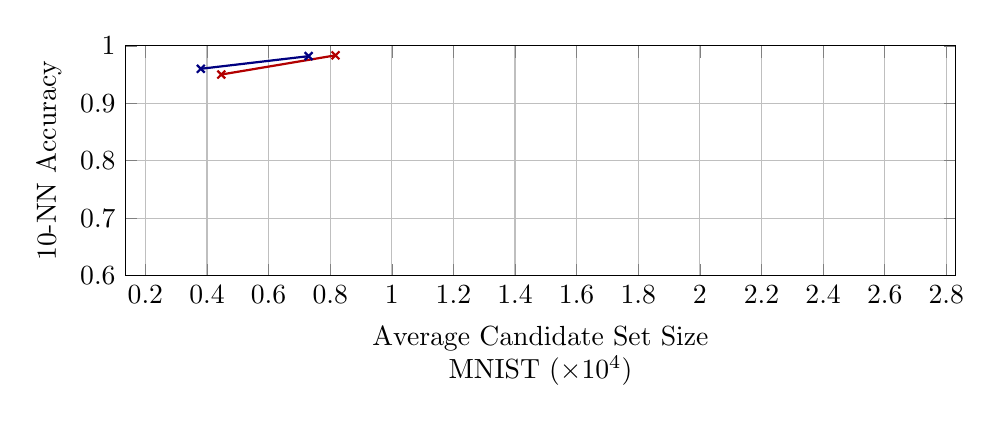
\begin{tikzpicture}
        \begin{axis}[
            width=\linewidth,
            height=4.5cm,
            grid=major,
            xlabel={\begin{tabular}{@{}c@{}}Average Candidate Set Size\\ MNIST ($\times 10^4$)\end{tabular}},
            ylabel={10-NN Accuracy},
            mark options={solid},
            xtick scale label code/.code={},
            xticklabel style={align=center},
            xmax=28299,
            ymin=0.6,
            ymax=1
        ]
        
        % Original
        \addplot[blue!50!black, thick, mark=x, mark size=2pt] coordinates {
            (3800, 0.96)
            (7300, 0.982)
        };
        % PCA
        \addplot[red!70!black, thick, mark=x, mark size=2pt] coordinates {
            (4465, 0.95)
            (8173, 0.9834)
        };        
        \end{axis}
\end{tikzpicture} % Make sure the individual plot does not include a legend
    \end{subfigure}
\end{figure}

    \begin{itemize}
        \item Achieved 1\% accuracy increase at candidate sizes of 190,000-195,000 on SIFT.
    	\item Reduced search time to 0.42 ms on SIFT, a 66\% improvement.
    	\item Exhibited similar performance to the original on MNIST.
    	\item Achieved 0.22 ms search time on MNIST, a 70\% reduction.
    \end{itemize}
    
\end{frame}

\begin{frame}{Results: \textcolor{MyOriginal}{Original}, \textcolor{MyPca}{PCA}, \textcolor{MyMahalanobis}{Mahalanobis}}
\begin{figure}[h]
    \centering    
    \begin{subfigure}[b]{0.45\textwidth}
        \centering
        \input{plots/sift-16b} % Make sure the individual plot does not include a legend
    \end{subfigure}
    \hspace{2mm}
    \begin{subfigure}[b]{0.45\textwidth}
        \centering
        \input{plots/mnist-16b} % Make sure the individual plot does not include a legend
    \end{subfigure}
\end{figure}

    \begin{itemize}
    	\item Matched PCA with 0.42 ms search time on SIFT, a 66\% improvement.
    	\item Reduced search time to 0.21 ms on MNIST, a 70\% improvement.
    \end{itemize}

\end{frame}

\begin{frame}{Results: \textcolor{MyOriginal}{Original}, \textcolor{MyPca}{PCA}, \textcolor{MyMahalanobis}{Mahalanobis}, \textcolor{MyCnn}{CNN}}
\begin{figure}[h]
    \centering    
    \begin{subfigure}[b]{0.45\textwidth}
        \centering
        \input{plots/sift-16c} % Make sure the individual plot does not include a legend
    \end{subfigure}
    \hspace{2mm}
    \begin{subfigure}[b]{0.45\textwidth}
        \centering
        \input{plots/mnist-16c} % Make sure the individual plot does not include a legend
    \end{subfigure}
    
    \begin{itemize}
    	\item Achieved high performance on MNIST with only 4-5 epochs, compared to 40+ epochs for linear models.
    \end{itemize}
    
\end{figure}

\end{frame}

\begin{frame}{Results: \textcolor{MyOriginal}{Original}, \textcolor{MyPca}{PCA}, \textcolor{MyMahalanobis}{Mahalanobis}, \textcolor{MyCnn}{CNN}, \textcolor{MyEnsembling}{Multi-Ensembling}}
\begin{figure}[h]
    \centering    
    \begin{subfigure}[b]{0.45\textwidth}
        \centering
        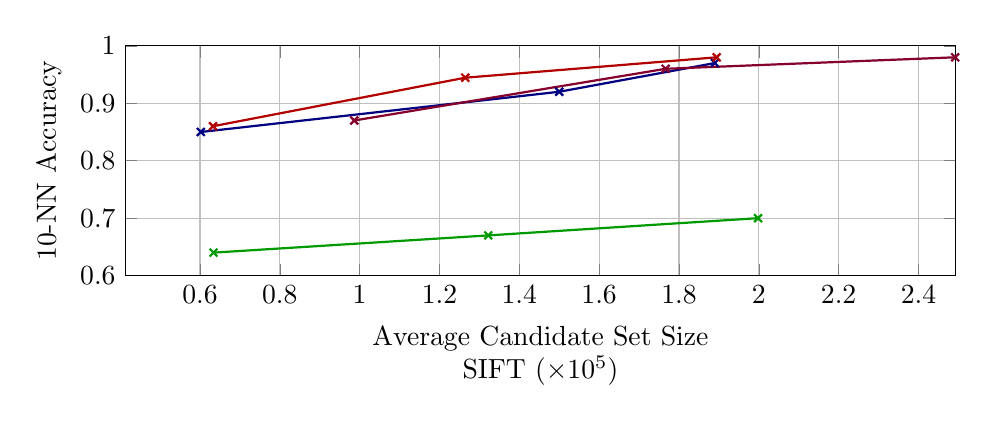
\begin{tikzpicture}
        \begin{axis}[
            width=\linewidth,
            height=4.5cm,
            grid=major,
			xlabel={\begin{tabular}{@{}c@{}}Average Candidate Set Size\\ SIFT ($\times 10^5$)\end{tabular}},
            ylabel={10-NN Accuracy},
            mark options={solid},
            xtick scale label code/.code={},
            xticklabel style={align=center},
            ymin=0.6,
            ymax=1,
            xmax=249300
        ]
        
        % Original
        \addplot[blue!50!black, thick, mark=x, mark size=2pt] coordinates {
            (60200, 0.85)
            (150000, 0.92)
            (189000, 0.97)
        };
        % PCA
        \addplot[red!70!black, thick, mark=x, mark size=2pt] coordinates {
            (63243, 0.86)
            (126475, 0.9445)
            (189444, 0.98)
        };
        % Mahalanobis
        \addplot[green!60!black, thick, mark=x, mark size=2pt] coordinates {
            (63386, 0.64)
            (132219, 0.67)
            (199818, 0.70)
        };
        % Multi-model ensembling 
        \addplot[purple!70!black, thick, mark=x, mark size=2pt] coordinates {
            (98631, 0.87)
            (176668, 0.96)
            (249204, 0.98)
        };
        \end{axis}
\end{tikzpicture} % Make sure the individual plot does not include a legend
    \end{subfigure}
    \hspace{2mm}
    \begin{subfigure}[b]{0.45\textwidth}
        \centering
        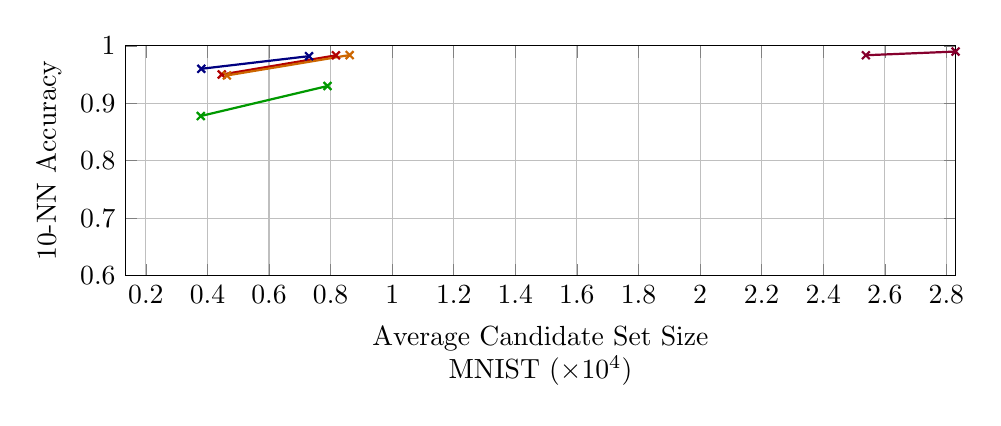
\begin{tikzpicture}
        \begin{axis}[
            width=\linewidth,
            height=4.5cm,
            grid=major,
            xlabel={\begin{tabular}{@{}c@{}}Average Candidate Set Size\\ MNIST ($\times 10^4$)\end{tabular}},
            ylabel={10-NN Accuracy},
            mark options={solid},
            xtick scale label code/.code={},
            xticklabel style={align=center},
            xmax=28299,
            ymin=0.6,
            ymax=1
        ]
        
        % Original
        \addplot[blue!50!black, thick, mark=x, mark size=2pt] coordinates {
            (3800, 0.96)
            (7300, 0.982)
        };
        % PCA
        \addplot[red!70!black, thick, mark=x, mark size=2pt] coordinates {
            (4465, 0.95)
            (8173, 0.9834)
        };
        % Mahalanobis
        \addplot[green!60!black, thick, mark=x, mark size=2pt] coordinates {
            (3784, 0.8778)
            (7899, 0.93)
        };
        % CNN 
        \addplot[orange!80!black, thick, mark=x, mark size=2pt] coordinates {
            (4631, 0.9484)
            (8618, 0.9839)
        };
        % Multi-model ensembling 
        \addplot[purple!70!black, thick, mark=x, mark size=2pt] coordinates {
            (25386, 0.9836)
            (28299, 0.99)
        };
        
        \end{axis}
\end{tikzpicture} % Make sure the individual plot does not include a legend
    \end{subfigure}
    
    \begin{itemize}
        \item Exhibited tendency of creating oversized partitions.
    	\item Demonstrated complexity in integrating different models for high-dimensional data.
    \end{itemize}
    
\end{figure}

\end{frame}


\begin{frame}{Conclusions}

\begin{block}{\centering \Large}
    \hspace{1cm}
    \begin{itemize}
        \item Achieved notable search time reductions with PCA and Mahalanobis; difficulties presented in handling high number of partitions
        \item Demonstrated CNNs' efficiency; achieved high performance with minimal epochs (original used 90+ with a neural network)
        \item Revealed multi-ensembling complexities; smarter functions for the combination of models are required (probabilistic, genetic algorithms)
        \item Proposed future steps in adaptive techniques, alternative loss functions, and hybrid model and  unsupervised space partitioning (hnsw and product vector quantisation)
    \end{itemize}
\end{block}

\end{frame}

\begin{frame}[allowframebreaks]{References}

  \bibliography{demo}
  \bibliographystyle{abbrv}

\end{frame}

\end{document}